\section{Results}
\label{sec:results}

\subsection{Single-model Translations}
In this section, we use two models: both are trained on the text of the English Wikipedia and the Dutch Wikipedia combined. The only difference between the two models is the number of dimensions: one is trained at 100, and the other at 400 dimensions.

Since the Dutch Wikipedia is much smaller than its English counterpart (by a factor of 8, see table~\ref{table:datasets}), we ran it eight times over the Dutch text. This artificially increases the weight given to Dutch text, so both are equally well represented.

\subsubsection{Single Model Using Single Relation}
The method described in section~\ref{sec:single-model-no-matrix} is tested by randomly selecting 100 translations from our testset of correct translations. These are used as a known translation, to derive other translations from. For each of these translations, we then select 500 different translations to test against. This process is done both for a model trained at 100 dimensions, and one trained at 400 dimensions, and both for Dutch to English and vice versa.

For example, given "koning $\to$ king" as base pair, we then test whether the algorithm can translate "koningin" to "queen", "kopen" to "buy", et cetera.

Table~\ref{table:results_single_model_no_matrix} shows the results of these experiments.

\begin{table}[ht!]
  \centering
  \label{table:results_single_model_no_matrix}
  \begin{tabular}{ll|r|r|r|r|}
  \cline{3-6}                                       &     & \multicolumn{2}{|c|}{100 dim} & \multicolumn{2}{c|}{400 dim} \\ \cline{3-6} 
                                                    &     & NL$\to$EN   & EN$\to$NL       & NL$\to$EN   & EN$\to$NL      \\ \hline
    \multicolumn{1}{|l|}{\multirow{3}{*}{Avg.}}     & @1  & 4.29\%      & 3.92\%          & 1.91\%      & 2.02\%         \\ \cline{2-6} 
    \multicolumn{1}{|l|}{}                          & @5  & 8.71\%      & 8.28\%          & 4.89\%      & 4.97\%         \\ \cline{2-6} 
    \multicolumn{1}{|l|}{}                          & @10 & 11.4\%      & 10.9\%          & 6.96\%      & 7.00\%         \\ \hline 
    \multicolumn{1}{|l|}{\multirow{3}{*}{Max.}}     & @1  & 14.6\%      & 12.4\%          & 8.60\%      & 8.60\%         \\ \cline{2-6} 
    \multicolumn{1}{|l|}{}                          & @5  & 23.4\%      & 23.8\%          & 15.8\%      & 16.4\%         \\ \cline{2-6} 
    \multicolumn{1}{|l|}{}                          & @10 & 28.4\%      & 28.6\%          & 21.2\%      & 22.0\%         \\ \hline
    \multicolumn{1}{|l|}{\multirow{3}{*}{Stdev.}}   & @1  & 3.50\%      & 3.24\%          & 1.97\%      & 2.19\%         \\ \cline{2-6} 
    \multicolumn{1}{|l|}{}                          & @5  & 6.10\%      & 6.15\%          & 4.11\%      & 4.55\%         \\ \cline{2-6} 
    \multicolumn{1}{|l|}{}                          & @10 & 7.51\%      & 7.60\%          & 5.42\%      & 5.85\%         \\ \hline
  \end{tabular}
  \caption{Translation accuracy, using a single model without translation matrix and 400 dimensions. The minimum is left out, because it is 0.00\% for all scenarios.}
\end{table}

An important note (which is not shown in the table), is that for every scenario, the lowest percentage of correct translations is 0.00\%. This means that there are some very bad base translations. In the next section, we will give some reasons what may cause this.

Overall, we can clearly see that this algorithm does not give good results. The best accuracy is below 25\%, compared to almost 75\% for algorithms using a translation matrix.

\subsubsection{Single Model Using Translation Matrix}
The single-model algorithm with translation matrix is tested exactly the same as the multi-model version. The results of the experiments are plotted in figure~\ref{fig:sm_100} and~\ref{fig:sm_400}. 

An interesting observation is that the accuracy at all levels (top 1, top 5 and top 10) starts off lower for models trained at 400 dimensions. However, at the biggest training set (2900 training pairs), the accuracy is better at all three levels, compared to the corresponding levels at 100 dimensions.

\begin{figure*}[!htb]
    \centering
    \begin{minipage}{\textwidth}
      \centering
      \begin{minipage}{0.45\linewidth}
          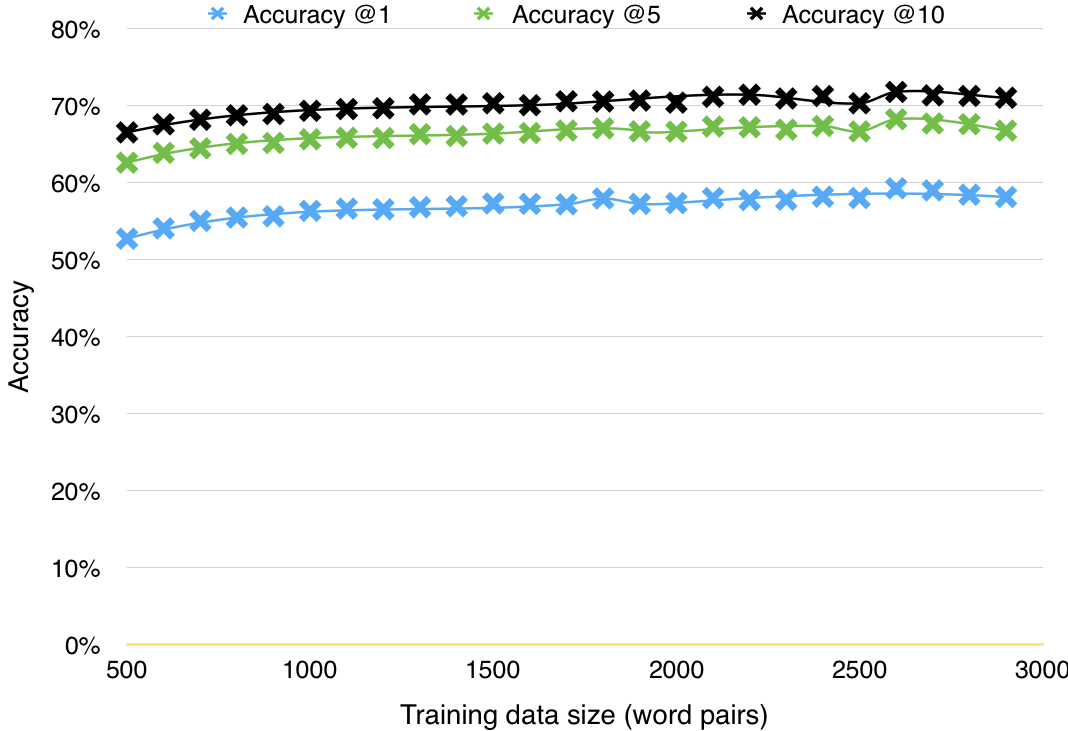
\includegraphics[width=\linewidth]{images/single_model_100_dim}
          \caption{Single model, 100 dimensions}
          \label{fig:sm_100}
      \end{minipage}
      \begin{minipage}{0.45\linewidth}
          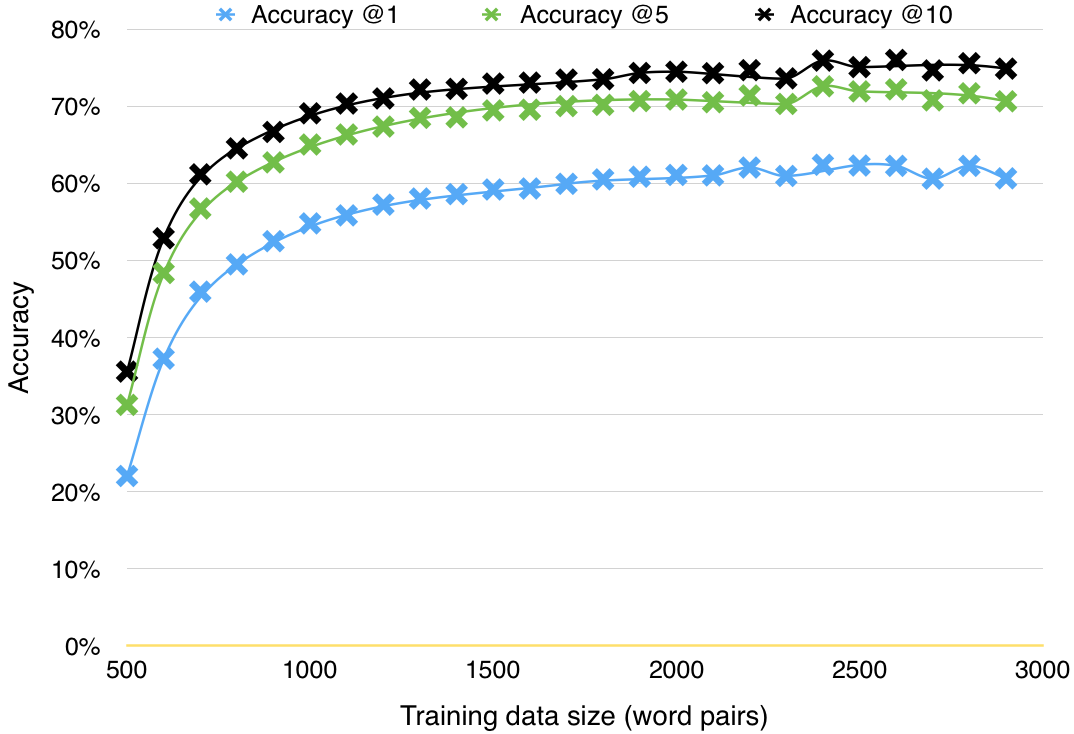
\includegraphics[width=\linewidth]{images/single_model_400_dim}
          \caption{Single model, 400 dimensions}
          \label{fig:sm_400}
      \end{minipage}
    \end{minipage}
\end{figure*}

\subsection{Multi-model Translations}
Figure~\ref{fig:sm_100} (resp.~\ref{fig:sm_400}) shows the accuracy of the multi-model translations, for models trained on 100 (resp. 400) dimensions. Table~\ref{table:graphdata} shows a selection of the data plotted in the graphs, to allow for easier comparison between the single model/multiple models and 100/400 dimensions. It only shows the accuracy for getting the answer exactly right (referred to as "@1").

\begin{figure*}[!htb]
    \centering
    \begin{minipage}{\textwidth}
      \centering
      \begin{minipage}{.45\textwidth}
          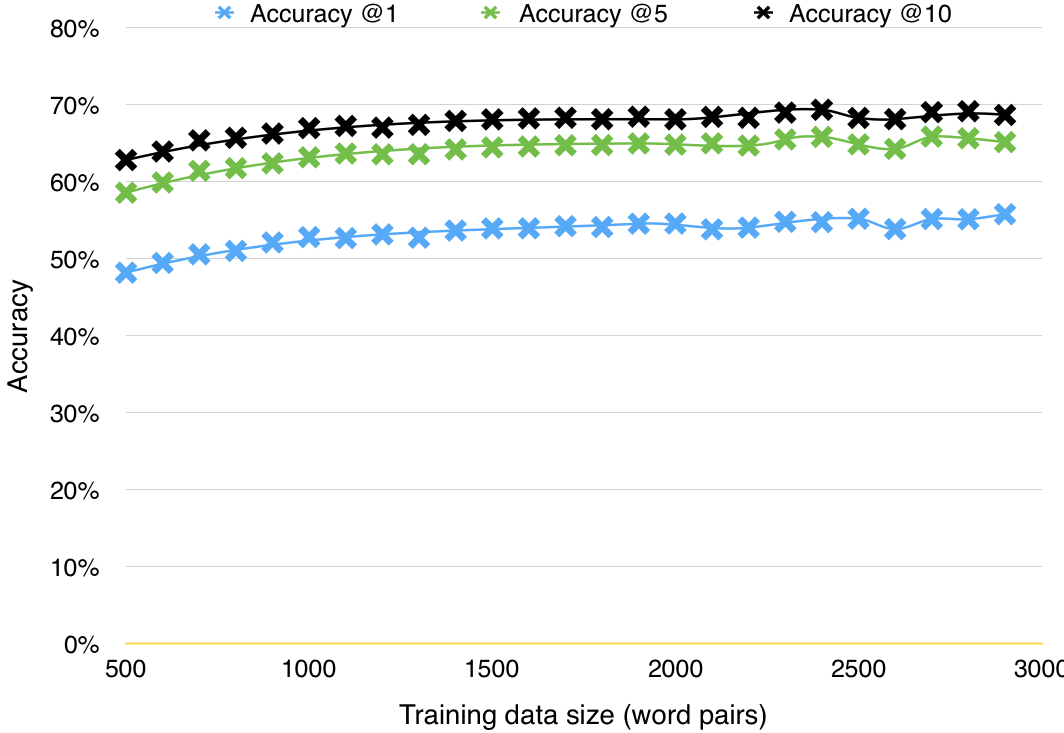
\includegraphics[width=\linewidth]{images/multiple_model_100_dim}
          \caption{Multiple models, 100 dimensions}
          \label{fig:mm_100}
      \end{minipage}
      \begin{minipage}{.45\textwidth}
          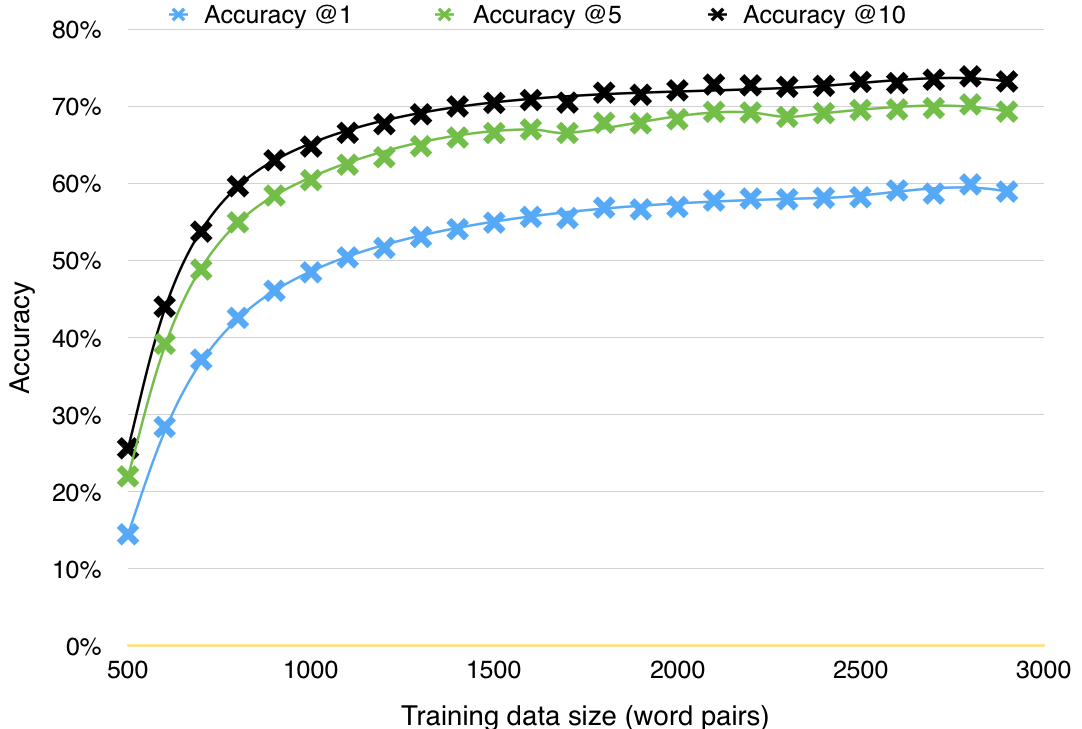
\includegraphics[width=\linewidth]{images/multiple_model_400_dim}
          \caption{Multiple models, 400 dimensions}
          \label{fig:mm_400}
      \end{minipage}
    \end{minipage}
\end{figure*}

Note that for small sets of training data (e.g. 500 translation pairs), the single model version of the algorithm is more accurate the multiple model version by roughly 5\%. For large sets of training data, the results are almost identical. We used the same set of training/test data for both experiments, to avoid any bias.

Also, we see once again that the 400 dimensional word2vec models require a larger set of translation pairs for training, but that they can perform better than the 100 dimensional models when given enough training data.

\begin{table}[]
  \centering
  \label{table:graphdata}
  \begin{tabular}{|l|l|l|l|l|}
    \hline
    \multirow{2}{*}{Training pairs} & \multicolumn{2}{l|}{Single model} & \multicolumn{2}{l|}{Multiple models} \\ \cline{2-5} 
                                    & 100 dim         & 400 dim         & 100 dim           & 400 dim          \\ \hline
    500                             & 53\%            & 22\%            & 48\%              & 14\%             \\ \hline
    1700                            & 57\%            & 60\%            & 54\%              & 55\%             \\ \hline
    2900                            & 58\%            & 61\%            & 56\%              & 59\%             \\ \hline
  \end{tabular}
  \caption{Accuracy for single and multi model, 100 and 400 dimensions. Only statistics for exact answers ("@1") are shown.}
\end{table}

% \begin{figure}[ht!]
%   \centering 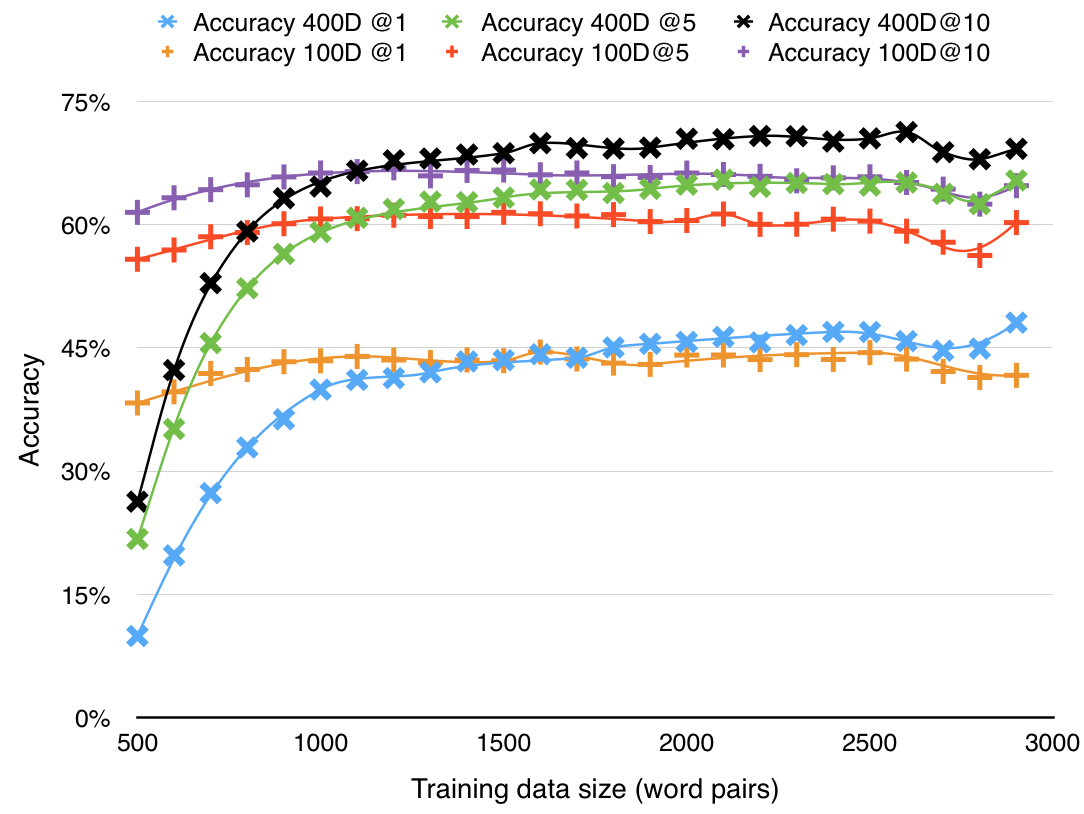
\includegraphics[width=\linewidth]{images/accuracy_multi_model_wikis}
%   \caption{Accuracy for multi-model translations, trained on Dutch and English wiki. 'x' marks denote dimensionality 400, '+' marks dimensionalty 100.}
%   \label{fig:accuracy_multi_model_wikis}
% \end{figure}
% \begin{figure}[ht!]
%   \centering 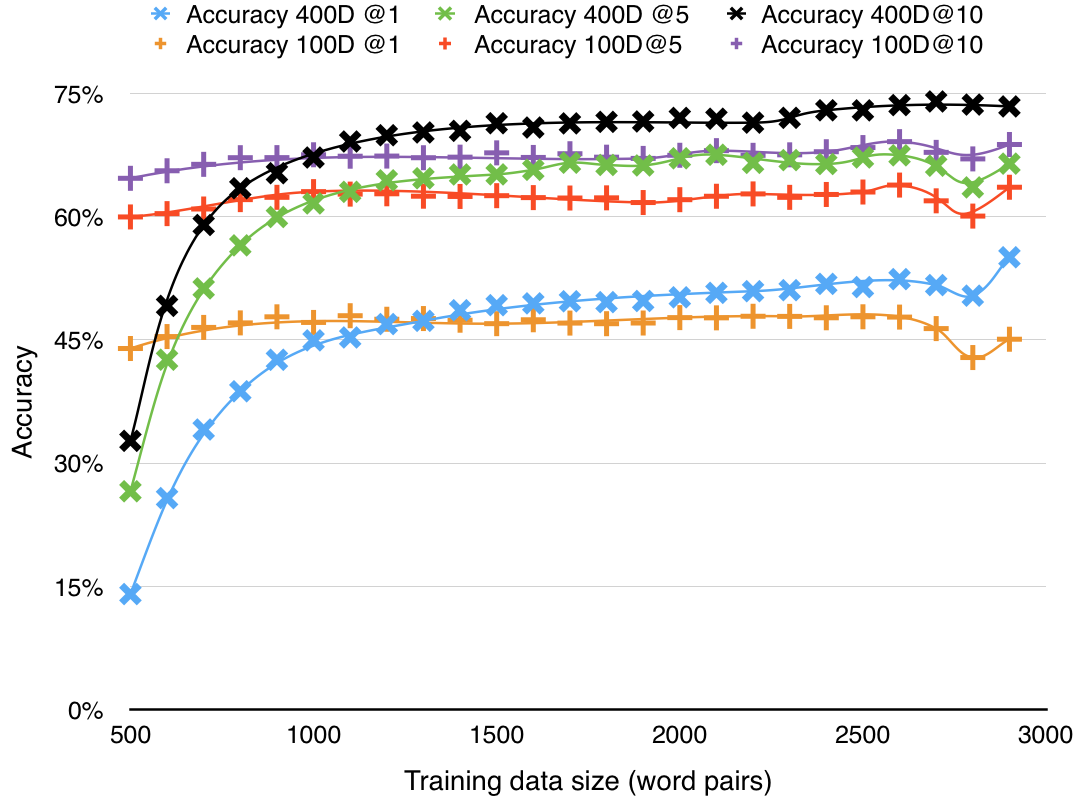
\includegraphics[width=\linewidth]{images/accuracy_single_model_wikis}
%   \caption{Accuracy for single-model translations, trained on Dutch and English wiki. 'x' marks denote dimensionality 400, '+' marks dimensionalty 100.}
%   \label{fig:accuracy_single_model_wikis}
% \end{figure}